\documentclass[10pt]{article}
\usepackage[publish]{dlmath}
\usepackage{tablefootnote}
\usepackage{marvosym}
\usepackage[hyphens]{url}
\usepackage[colorlinks=true, linkcolor=blue]{hyperref}
\usepackage{makeidx}
\newcommand{\dom}[1]{\ensuremath{\hbox{Dom}(#1)}}
%\newcommand{\code}[1]{\texttt{#1}}

%{\theoremstyle{definition} \newtheorem{note}{Note}}
%\newtheorem{defn}{Definition}
%opening
\title{Piecewise Linear with Decay}
\author{Bill Adams}
\date{Sept 2020}
\makeindex

\begin{document}
\maketitle

\tableofcontents
%\begin{abstract}
%\end{abstract}

%\tableofcontents

\section{Introduction}
A piecewise defined function is a function whose formula varies on different
regions of the domain. Typically those regions are continuous intervals, i.e.
sets of the form
$$[a,b] \defeq \{x | a \leq x \leq b\}$$
or
$$(a,b) \defeq \{x | a < x < b\}$$
or some mixture of half-closed and half-opened intervals.

The best way to get a feel for piecewise defined functions is to see an
example and the corresponding graph of the function.
Consider the following piecewise defined function examples:
\begin{note}
In the graphs below We use the red dots to indicate the beginning
and end points of the domains of definition of the function.
\end{note}
\begin{example}
\label{ex:1}
$$
f(x) =
\begin{cases}
x^2 & \hbox{ if } x\in [0,2] \\
-x+6 & \hbox{ if } x \in [2, 5]
\end{cases}
$$
\begin{center}
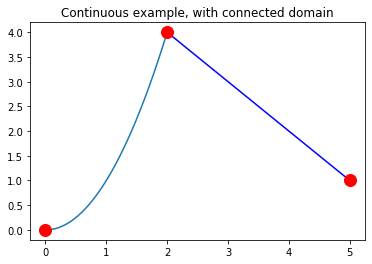
\includegraphics[width=2.5in]{graph1}
\end{center}
The function $f(x)$ is only defined on the closed interval $[0, 5]$, that is
we can only calculate $f(x)$ for values of $x$ between 0 and 5.  The function
is continuous, that is we can draw the graph without picking up our pencil.
Also the domain of the function, namely $x \in [0,5]$ is connected.
\end{example}
\begin{example}
\label{ex:2}
$$
f(x) =
\begin{cases}
x^3 & \hbox{ if } x\in [0,2] \\
x-2 & \hbox{ if } x \in (2, 5]
\end{cases}
$$
\begin{center}
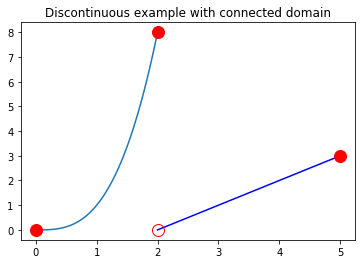
\includegraphics[width=2.5in]{graph2}
\end{center}
This is an example of a discontinuous piecewise defined function because the
graph has a break over $x=2$.  Note that the first definition covers the
closed interval $[0,2]$ whereas the second definition only covers the
half-opened interval $(2,5]$.  However this function has a domain of
$x \in [0, 5]$ which is a connected domain (there are no gaps in it).
\end{example}

\begin{example}
\label{ex:3}
$$
f(x) =
\begin{cases}
x^3 & \hbox{ if } x\in [0,2] \\
x-2 & \hbox{ if } x \in [5, 8]
\end{cases}
$$
\begin{center}
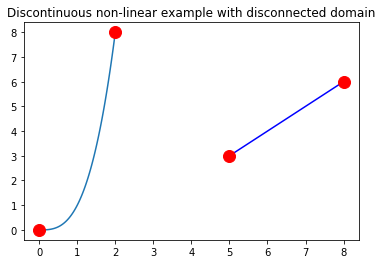
\includegraphics[width=2.5in]{graph3}
\end{center}
This is an example of a discontinuous piecewise defined function because the
graph has a break from $x=2$ to $x=5$.  Also his function has a domain of
$x \in [0, 2] \cup [5,8]$ which is a disconnected domain, i.e.
there is a gap in the domain from $2$ to $5$.
\end{example}

For the purposes of this paper we only consider piecewise defined functions
that are continuous and have a connected domain.  In other words we only
consider the case of Example \ref{ex:1}.  We do not consider discontinuous
piecewise defined functions like Example \ref{ex:2}.  Neither do we consider
piecewise defined functions whose domain is disconnects, as in Example
\ref{ex:3}.
\section{Piecewise linear functions}
A piecewise linear function is simply a piecewise defined function whose
every piece is a linear function.  There are several ways we could formally
define this.  The following is a more abstract definition.
\begin{definition}
A function $f(x)$ is a \ul{piecewise linear, continuous function, with
finite connected domain} iff:
\begin{enumerate}
\item $f(x)$ is continuous
\item The domain of $f(x)$, which we write as \dom{f}, is a finite connected
interval.  In other words, it does not go to infinity on either side.
\item For every point $x_0 \in \dom{f}$ there is an interval $[a,b]$ so that
$x \in [a,b]$ and $f(x)$ restricted to $[a,b]$ is a linear function.
\end{enumerate}
\end{definition}
\begin{note}
We only consider piecewise linear, continuous functions with connected domain.
Thus we shorten that long phrase to \ul{piewewise linear function}.
\end{note}
A more concrete definition of a piecewise linear function is the following.
\begin{definition}[Concrete definition of piecewise linear]
\label{def:concrete}
A function $f(x)$ is a \ul{piecewise linear function} iff it can be written as
$$f(x) =
\begin{cases}
m_1 x + b_1 & \hbox{ if } x \in [a_1, a_2] \\
m_2 x + b_2 & \hbox{ if } x \in [a_2, a_3] \\
\vdots & \vdots \\
m_{n-1} x + b_{n-1} & \hbox{ if } x \in [a_{n-1}, a_n]
\end{cases}
$$
where $a_1 < a_2 < \ldots < a_n$.
\end{definition}
\begin{note}
These two definitions are equivalent.  The second definition is much more
useful for computational purposes, the first would be more useful for the
purposes of proving things.
\end{note}
\begin{note}
\label{note:mb}
In Definition \ref{def:concrete}, the slope $m_i$ and y intercept $b_i$ in
the function definition on the interval $[a_i, a_{i+1}]$ can be calculated by
knowing $y_i = f(a_i)$ and $y_{i+1}=f(a_{i+1})$.  We can show the formula by
noting that the function is linear from the point $(a_i, y_i)$ to the point
$(a_{i+1}, y_{i+1})$.  Then the slope $m_i$ is:
$$m_i = \frac{y_{i+1}-y_i}{a_{i+1}-a_i}$$
and $b_i$ can be found by plugging either point into the equation of the line
$y=mx+b$ and solving for $b$.  If we use $(a_i, y_i)$ we get:
$$b_i=y_i-ma_i$$
\end{note}
Based Note \ref{note:mb} we see that a piecewise linear function can be defined
by giving a list of $a_i$'s and $y_i$'s.  Therefore we have a simply computational
definition of a piecewise linear function.
\begin{definition}[Computational]
\label{def:computational}
A piecewise linear function is defined by $\vec{a}=(a_1,a_2,\ldots,a_n)$ and
$\vec{y}=(y_1, y_2, \ldots y_n)$, where $a_1<a_2<\ldots <a_n$.  The formula
for the piecewise linear function defined by $\vec{a}$ and $\vec{y}$ is given by
$$
f_{\vec{a},\vec{y}}(x) \defeq
\begin{cases}
m_1 x + b_1 & \hbox{ if } x \in [a_1, a_2] \\
m_2 x + b_2 & \hbox{ if } x \in [a_2, a_3] \\
\vdots & \vdots \\
m_{n-1} x + b_{n-1} & \hbox{ if } x \in [a_{n-1}, a_n]
\end{cases}
$$
where:
\begin{eqnarray*}
m_i &=& \frac{y_{i+1}-y_i}{a_{i+1}-a_i} \\
b_i &=& y_i - m x_i
\end{eqnarray*}
\end{definition}
\section{Piecewise linear with decay}
Given a piecewise linear function (that is continuous with connected finite
domain), is there a natural way to extend it to positive and negative infinity
given asymptotes on both sides?  For example consider the graph shown below:

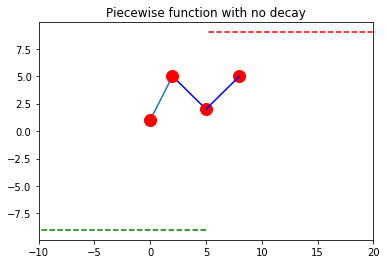
\includegraphics[width=2.5in]{pw_nodecay}

The red dotted line on top represents the asymptote on the right and the green
dotted line on the bottom represents the asymptote to the left.  Can we extend
our function continuously so that the graph approaches the given asymptotes?
There are many ways we can, consider:

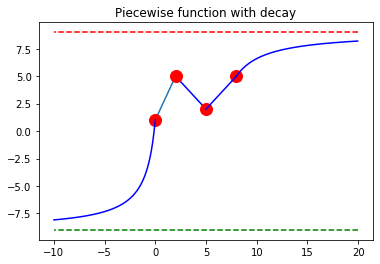
\includegraphics[width=2.5in]{pw_decay1a}

This graph extends the previous one with the desired asymptotic behavior.
However there are many other choices as well.  Looking at the graph above
notice that the slope of the graph where the left hand decay begins does
not match the slope of the piecewise linear piece beside it.  If we want
the slope of the decay function to match the slope of the linear piece the
decay connects with, this limits our choices more.  In fact if we:
\begin{enumerate}
\item specify the decay function to use (e.g. linear, exponential, etc), and
\item specify the resulting function must be continuous, and
\item specify that the slopes of the decays must match the slope of the piecewise linear
function on the edges of the domain \ldots
\end{enumerate}
then we uniquely determine the formula for the decay function to use.  Let's
collect that idea in Definition \ref{def:pwdecay}.  However first we need to
define the formulas for our decay functions.
\begin{definition}[Decay functions]
We define the exponential decay function as:
$$\mathfrak{e}_B(x) \defeq Ae^{Bx}+C$$
and we define the power decay function of degree $n$ as:
$$\mathfrak{p}_{k,B}(x) \defeq \frac{A}{(x-B)^k}+C$$
\end{definition}
\begin{note}
The parameter $C$ in both decay functions represents the limiting value
the function is decaying towards.
\end{note}
\begin{definition}
\label{def:pwdecay}
Given $f(x)$ a piecewise linear function (continuous on a finite connected domain $[a,b]$) and
\begin{enumerate}
\item a left hand asymptotic value $y_{-\infty}$
\item a right hand asymptotic value $y_{\infty}$
\item a decay function type (either exponential for fixed $b$, or power for fixed $b$ and $k$)
\end{enumerate}
an \ul{extension with decay} of $f(x)$ with decay is a function $\overline{f}(x)$ that:
\begin{enumerate}
\item the extension $\overline{f}$ agrees with $f$ on the domain $[a,b]$
\item the extension restricted to $(-\infty, a]$ matches the decay function type
\item the extension restricted to $[b, \infty)$ matches the decay function type
\item the extension is continuous
\item the slope of the extension at the points $x=a$ and $x=b$ are well defined.
\end{enumerate}
\end{definition}

We now have our main result:
\begin{theorem}
\label{thm:main}
Given a piecewise linear function (continuous on a finite connected domain $[a,b]$) such
that the slope at $x=a$ is not zero, and similarly for $x=b$, and
\begin{enumerate}
\item a left hand asymptotic value $y_{-\infty}$
\item a right hand asymptotic value $y_{\infty}$
\item a decay function type (either exponential for fixed $B$, or power for fixed $B$ and $k$)
\end{enumerate}
then there exists a unique extension with decay $\overline{f}$ of $f$.
\end{theorem}
We prove this theorem by proving the two cases separately
\begin{proof}
Proven in 2 cases, Theorem \ref{thm:power} and \ref{thm:exponential}.
\end{proof}

\begin{theorem}[Power Decay Version of Theorem \ref{thm:main}]
\label{thm:power}
Theorem \ref{thm:main} is true when the decay function is a power function, i.e.
$\mathfrak{p}_{k,B}(x)$.  Furthermore the parameters for the decay function on the left hand
side decay function is given by:
\begin{eqnarray*}
B&=&a_1 + \frac{k}{m_1}(y_1-B)\\
A&=&(y_1-C)(a_1-B)^k
\end{eqnarray*}
and the parameters for the right hand side decay function are given by:
\begin{eqnarray*}
B&=&a_n + \frac{k}{m_{n-1}}(y_n-B)\\
A&=&(y_n-C)(a_n-B)^k
\end{eqnarray*}
Where $\vec{a}=(a_1, \ldots, a_n)$, $\vec{y}=(y_1,\ldots,y_n)$ and $m_i$ are
as Definition \ref{def:computational}.
\end{theorem}
\begin{proof}
We need only derive the formula for $B$ and $A$ given that we know the value
of the decay function at point $x_0$ and the value of its derivative
at $x_0$ and the limiting value, which is $C$.  So given our decay function:
\begin{eqnarray}
\label{eqn:1}
\mathfrak{p}_{k,B}(x)&=&\frac{A}{(x-B)^k} + C
\end{eqnarray}
and assume we know:
\begin{eqnarray}
\label{eqn:2}\mathfrak{p}_{k,B}(x_0)&=&y_0 \\
\label{eqn:3}\mathfrak{p}'_{k,B}(x_0)&=&m_0 \\
C&=&\hbox{ the limiting value}
\end{eqnarray}
we want to use those equations to solve for $A, B$. Notice that:
\begin{eqnarray}
\label{eqn:4}\mathfrak{p}'_{k,B}(x) &=& \frac{-kA}{(x-B)^{k+1}}
\end{eqnarray}
Using Equation \ref{eqn:2} and the definition in Equation \ref{eqn:1} we get:
\begin{eqnarray}
\mathfrak{p}_{k,B}(x_0)&=&y_0 \\
\frac{A}{(x_0-B)^k} +C &=& y_0 \\ \label{eqn:k}
\frac{A}{(x_0-B)^k} &=& y_0 - C
\end{eqnarray}
Using Equation \ref{eqn:3} and the definition of the slope in Equation
\ref{eqn:4} we see:
\begin{eqnarray}
\mathfrak{p}'_{k,B}(x_0)&=&m_0 \\
\frac{-kA}{(x_0-B)^{k+1}}&=&m_0 \\
\left(\frac{A}{(x_0-B)^{k}}\right) \left( \frac{-k}{x_0-B} \right) &=&m_0 \\
\hbox{plug Equation \ref{eqn:k} in} \\
\left(y_0-C\right)\left( \frac{-k}{x_0-B} \right) &=& m_0 \\
y_0-C &=& -(x_0-B)\frac{m_0}{k} \\
(y_0-C)\frac{k}{m_0}&=&-x_0+B \\
\label{eqn:Bsolve}(y_0-C)\frac{k}{m_0}+x_0&=&B
\end{eqnarray}
With this we have solved for $B$, now we need to solve for $A$.  We can use
Equation \ref{eqn:k} to do this.
\begin{eqnarray}
\frac{A}{(x_0-B)^k} &=& y_0 - C \\
\label{eqn:Asolve} A &=& (x_0-B)^k(y_0-C)
\end{eqnarray}
Using Equations \ref{eqn:Bsolve} and \ref{eqn:Asolve} for $x_0=a_1, y_0=y_1, m_0=m_1$ we
get the left side decay formula for $A$ and $B$.  Similarly using those equations for
$a_n, y_n, m_{n-1}$ we get the right side decay formula for $A$ and and $B$.
\end{proof}

\begin{theorem}[Exponential Decay Version of Theorem \ref{thm:main}]
\label{thm:exponential}
Theorem \ref{thm:main} is true when the decay function is an exponential function, i.e.
$\mathfrak{e}_{B}(x)$.  Furthermore the parameters for the decay function on the left hand
side decay function is given by:
\begin{eqnarray*}
A&=&(y_1-C)e^{-Ba_1}\\
B &=& \frac{m_1}{y_1-C}
\end{eqnarray*}
and the parameters for the right hand side decay function are given by:
\begin{eqnarray*}
A&=&(y_n-C)e^{-Ba_n}\\
B &=& \frac{m_{n-1}}{y_n-C}
\end{eqnarray*}
Where $\vec{a}=(a_1, \ldots, a_n)$, $\vec{y}=(y_1,\ldots,y_n)$ and $m_i$ are
as Definition \ref{def:computational}.
\end{theorem}
\begin{proof}
As with the proof of Theorem \ref{thm:power} we simply need to prove the
formulas for $A$ and $C$ when we have the conditions
\begin{eqnarray}
\mathfrak{e}_{B}(x_0) &=& y_0 \label{eqn:e1}\\
\mathfrak{e}'_{B}(x_0) &=& m_0 \label{eqn:e2}
\end{eqnarray}
Notice that the exponential decay function and its derivative are given by:
\begin{eqnarray}
\mathfrak{e}_{B}(x) = Ae^{Bx}+C \label{eqn:e3}\\
\mathfrak{e}'_{B}(x) = ABe^{Bx} \label{eqn:e4}
\end{eqnarray}
We can use the formula in Equation \ref{eqn:e3} and plug into Equation \ref{eqn:e1}
and get:
\begin{eqnarray}
\mathfrak{e}_{B}(x_0) &=& y_0 \\
Ae^{Bx_0} + C &=& y_0 \\
Ae^{Bx_0} &=& y_0 - C \label{eqn:ePlugin}\\
A&=&(y_0-C)e^{-Bx_0} \label{eqn:eAsolve}
\end{eqnarray}

Using the formula from Equation \ref{eqn:e4} with Equation \ref{eqn:e2} and
solving for $A$ we get:
\begin{eqnarray}
\mathfrak{e}'_{B}(x_0) &=& m_0 \\
ABe^{Bx_0} &=& m_0 \\
B \left(Ae^{Bx_0} \right)&=& m_0 \\
B(y_0-C) &=&m_0 \hbox{ (plugin Equation \ref{eqn:ePlugin})} \\
B &=& \frac{m_0}{y_0-C} \label{eqn:eBsolve}
\end{eqnarray}

We can use Equations \ref{eqn:eAsolve} and \ref{eqn:eBsolve} when $x_0=a_1$,
$y_0=y_1$ and $m_0=m_1$ to get the formulas for the left hand side decay formulas
for $A$ and $C$:
\begin{eqnarray*}
A&=&(y_1-C)e^{-Ba_1}\\
B &=& \frac{m_1}{y_1-C}
\end{eqnarray*}
And similarly we get the equations for the right hand side decay formula.
\end{proof}
%\bibliography{programming}
%\bibliographystyle{plain}
\end{document}
